{\usebackgroundtemplate{
    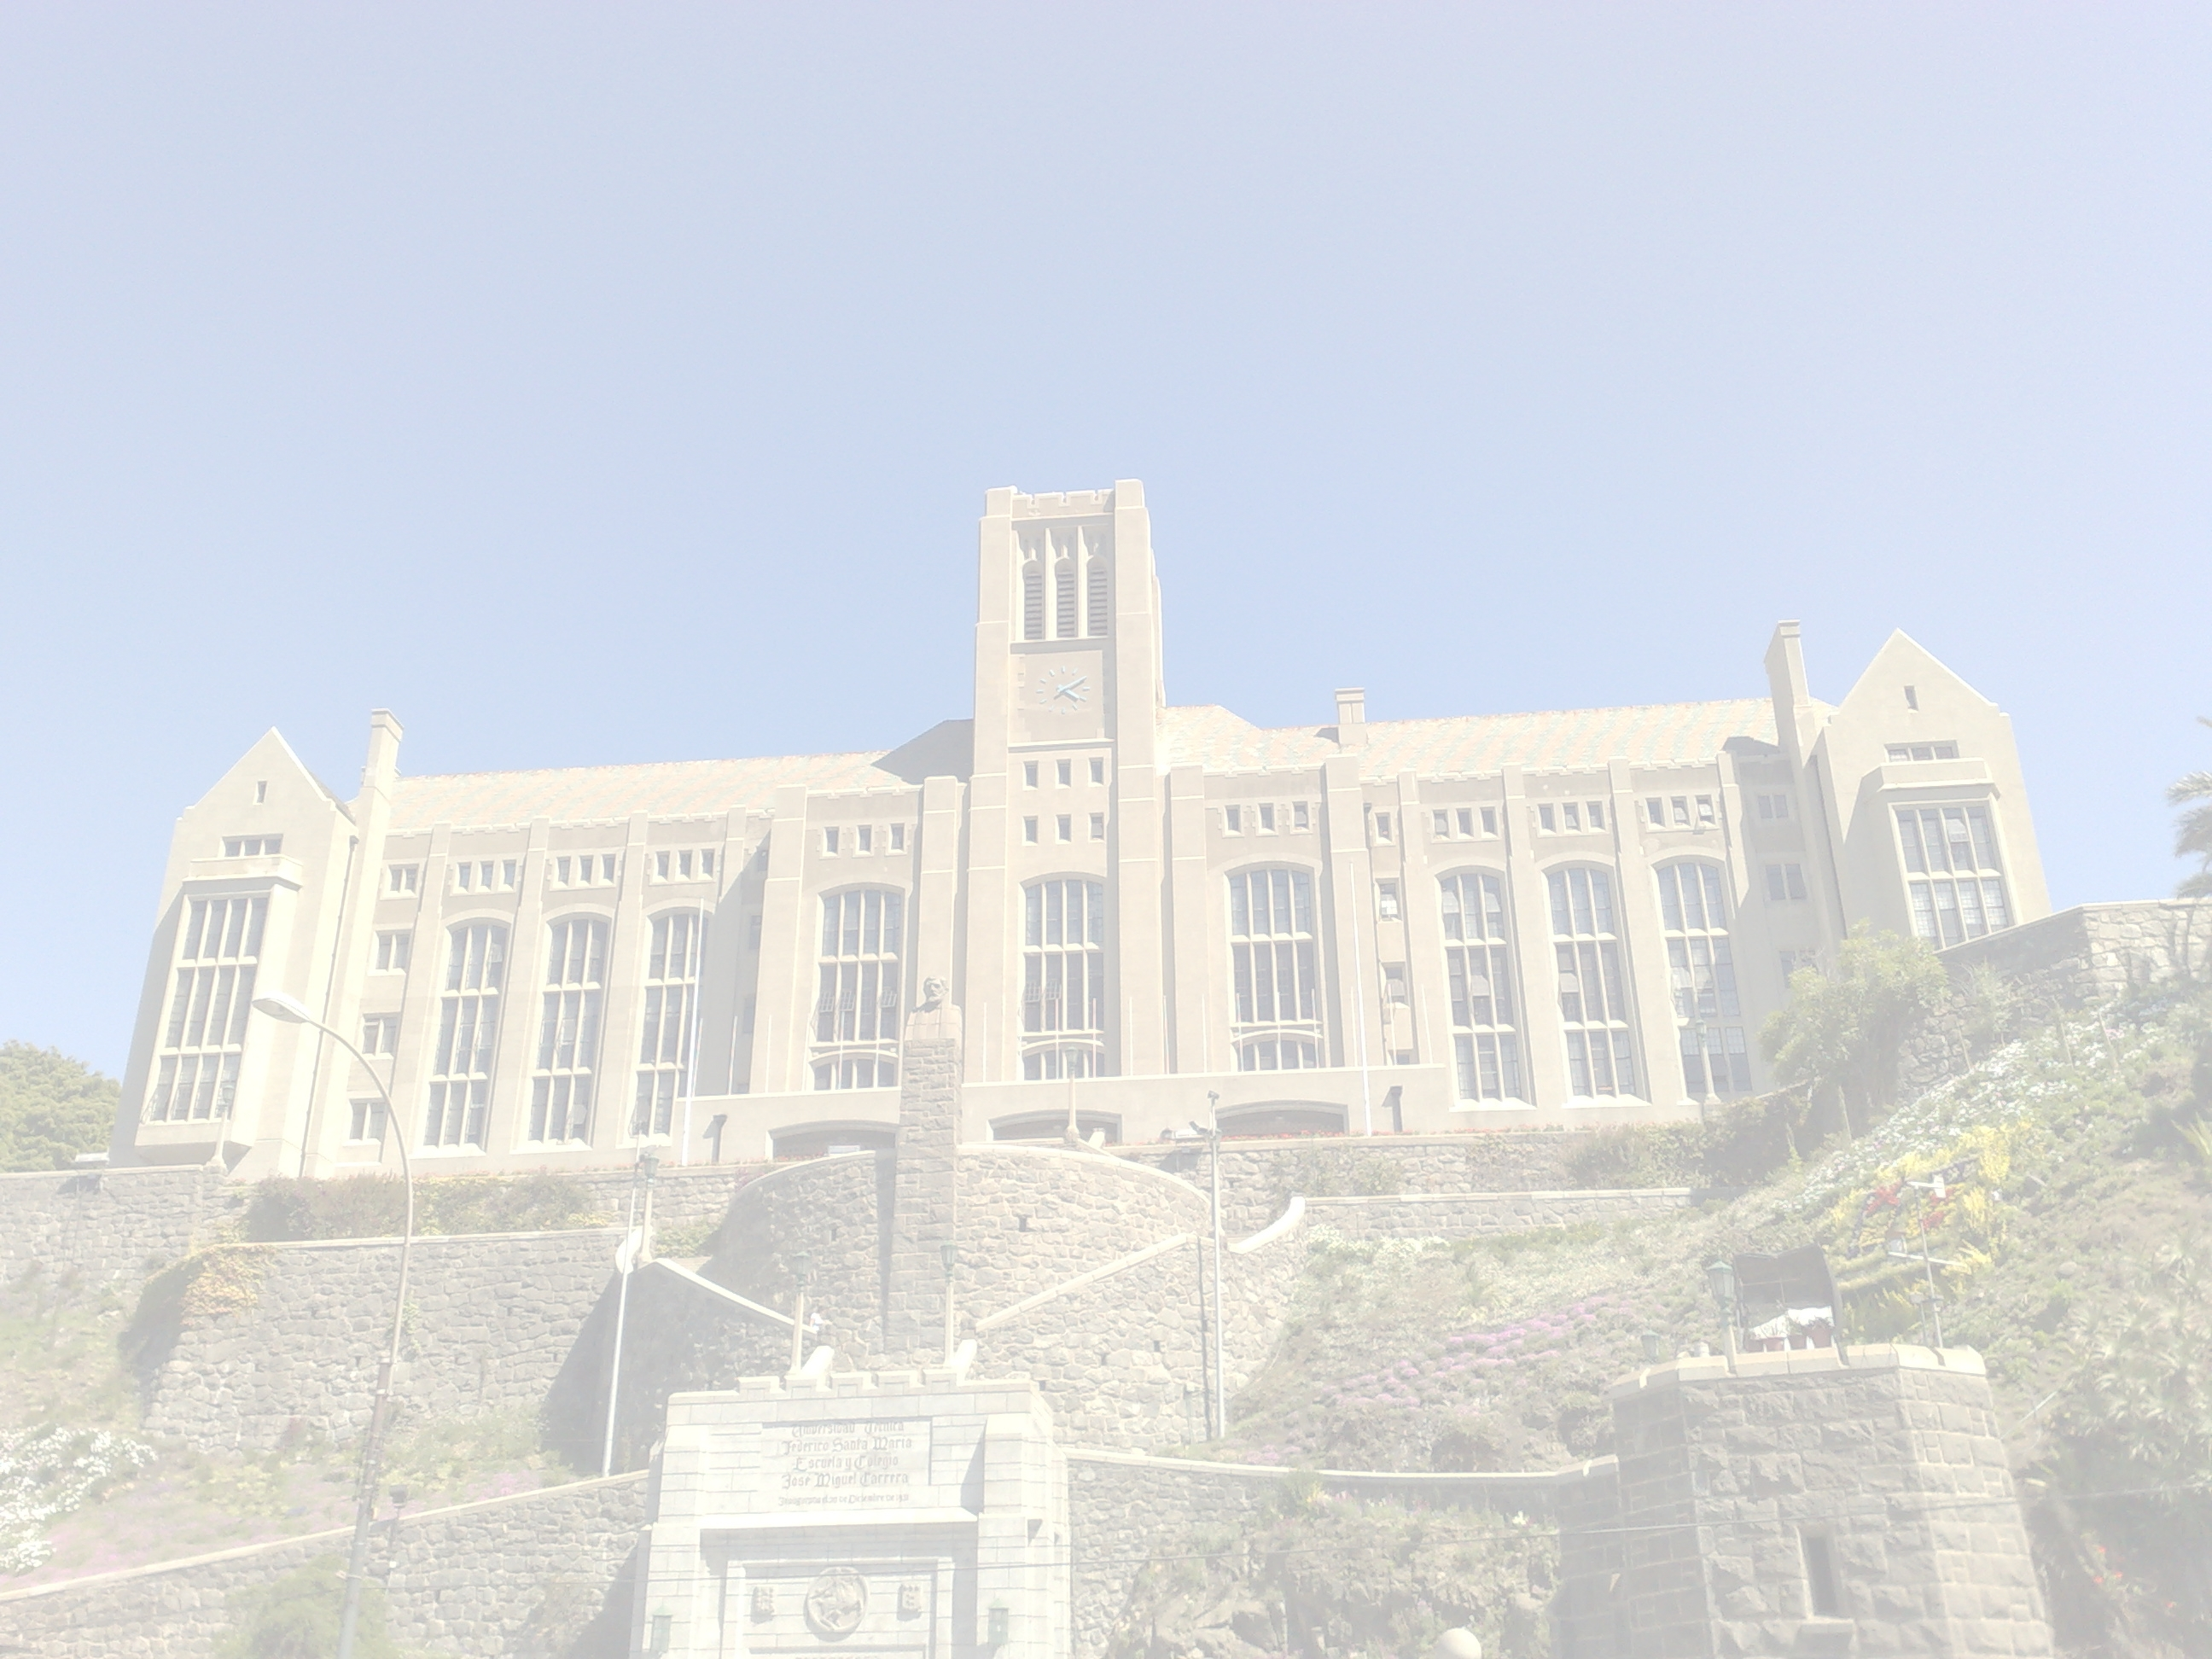
\includegraphics[width=\paperwidth,
      height=\paperheight]{Pict/UTFSM-30.jpg}
  }
  \begin{frame}
    \titlepage
  \end{frame}
}

\section{Algebraic Structures}

\begin{frame}
  \frametitle{Sets}
  \begin{definition}
    A \alert{set} is a collection of objects that do not necessarily have any additional structure or properties.
  \end{definition}
\end{frame}

\begin{frame}
  \frametitle{Groups}
  \begin{definition}
    A \alert{group} is  a pair, $(G,\circ)$, where $G$ is a set and ``$\circ$'' is an operation called group multiplication, satisfying:
    \begin{enumerate}[I]
    \item \uline{Closure}: $\forall\,g_1,g_2\in G,\rightarrow\;g_1\circ g_2\in G.$
    \item \uline{Associativity}: $g_1\circ (g_2 \circ g_3) = (g_1\circ g_2) \circ g_3.$
    \item \uline{Existence of Identity}: $\exists!\, e\in G$ s.t. $\forall\, g\in G,\; g\circ e= e\circ g = g$.
    \item \uline{Unique Inverse}: $\forall\, g\in G\; \exists!\, g^{-1}\in G$ s.t. $g\circ g^{-1} = g^{-1}\circ g = e.$
    \end{enumerate}
  \end{definition}

  A group is called \alert{Abelian} if additionally its product is commutative.
\end{frame}

\begin{frame}
  \frametitle{Field}
  \begin{definition}
    A \alert{field}, $F$, is a triplet $(F,+,\circ)$ satisfying:
    \begin{enumerate}[I]
    \item $F$ is an Abelian group under $+$.
    \item Under the action of $\circ$ satisfy
      \begin{enumerate}[i]
      \item \uline{Closure}: $f_1\circ f_j \;\in\,F$.
      \item \uline{Associativity}: $f_1\circ (f_2 \circ f_3) = (f_1\circ f_2) \circ f_3.$
      \item \uline{Existence of Identity}: $\exists!\, 1\in F$ s.t. $\forall\, f\in G,\; f\circ 1= 1\circ f = f$.
      \item \uline{Unique Inverse}: $\forall\, (f\neq e)\in F\; \exists!\, f^{-1}\in F$ s.t. $f\circ f^{-1} = f^{-1}\circ f = 1.$
      \item \uline{Distributivity}: $f_i\circ (f_j + f_k) = f_i\circ f_j + f_i\circ f_k.$
      \end{enumerate}
    \end{enumerate}
  \end{definition}

  If the operation $\circ$ is commutative, the field is said to be commutative.
\end{frame}

\begin{frame}
  \frametitle{Linear Vector Space}
  \begin{definition}
    A \alert{linear vector space}, $V$, consists of $(V,F,+,\circ)$ with $V$ a collection of objects, $\{v_i\}$, called vectors, a field $F$, a vector addition $+$ and a scalar multiplication $\circ$, satisfying:
    \begin{enumerate}[I]
    \item $(V,+)$ is an Abelian group.
    \item The scalar multiplication satisfies:
      \begin{enumerate}[i]
      \item \uline{Closure}: $(f_i\circ v_j)\in\, V$.
      \item \uline{Associativity}: $f_1\circ (f_2 \circ v_3) = (f_1\circ f_2) \circ v_3.$
      \item \uline{Existence of Identity}: $1\circ v_i = v_i \circ 1 = v_i$.
      \item \uline{Bilinearity}: $f_i\circ (v_j + v_k)=f_i\circ v_j + f_i\circ v_k$.\\
        $(f_i + f_j)\circ v_k = f_i\circ v_k + f_j\circ v_k.$
      \end{enumerate}
    \end{enumerate}
  \end{definition}
\end{frame}

\begin{frame}
  \frametitle{Algebras}

  \begin{definition}
    A \alert{linear algebra}, $A$, is a collection $(V,F,+,\circ,\times)$, where $V$ is a vector space over $F$ under the operations $+,\circ$, and additionally, the $\times$ product satisfies:
    \begin{enumerate}[I]
    \item \uline{Closure}: $(v_i\times v_j)\in V$.
    \item \uline{Bilinearity}: $v_i\times(v_j+v_k) = v_i\times v_j + v_i\times v_k $\\
      $(v_i+v_j)\times v_k = v_i\times v_k+v_j\times v_k$
    \end{enumerate}
  \end{definition}
\end{frame}

\begin{frame}
  \frametitle{More About Algebras}
  \begin{itemize}
  \item An algebra is said to be associative if $(v_i\times v_j)\times v_k = v_i\times (v_j\times v_k)$.
  \item An algebra with identity is that which have an identity vector, $\mathds{1}$, s.t. $ v_i\times\mathds{1} = v_i$.
  \item If the vector multiplication satisfies, $v_i\times v_j =\pm v_j\times v_i$, the algebra is  said to be symmetric (antisymmetric) under interchange.
  \item If $v_i\times (v_j\times v_k) = (v_i\times v_j)\times v_k + v_j\times (v_i\times v_k)$ is satisfied, the algebra is said to posses derivative property.
  \end{itemize}
\end{frame}


\section{Manifolds}

\begin{frame}
  \frametitle{Manifolds}

  \begin{definition}
    $\Mi$ is a differential manifold if:
    \begin{enumerate}[i]
    \item $\Mi$ is a topological space.
    \item $\Mi$ is provided with an atlas, $\{(U_i,\varphi_i)\}$, which covers $\Mi$ and every $\varphi_i$ is a homeomorphism from $U_i$ onto an open subset of $\R^n$.
    \item For $U_i\cap U_j\neq \emptyset$, the map $\psi_{ij}=\varphi_i\circ\varphi_j^{-1}$ is $C^\infty$
    \end{enumerate}
  \end{definition}
\end{frame}

\begin{frame}
  \frametitle{Manifolds (examples)}
  %% \begin{definition}
  %%   A \alert{\bf Manifold}, $\Mi$, is a space locally homeomorphic to $\R^n$, for some $n$. The dimension of $\Mi$ is $n$.
  %% \end{definition}
  \begin{columns}
    \column{.5\textwidth}
    \begin{center}
      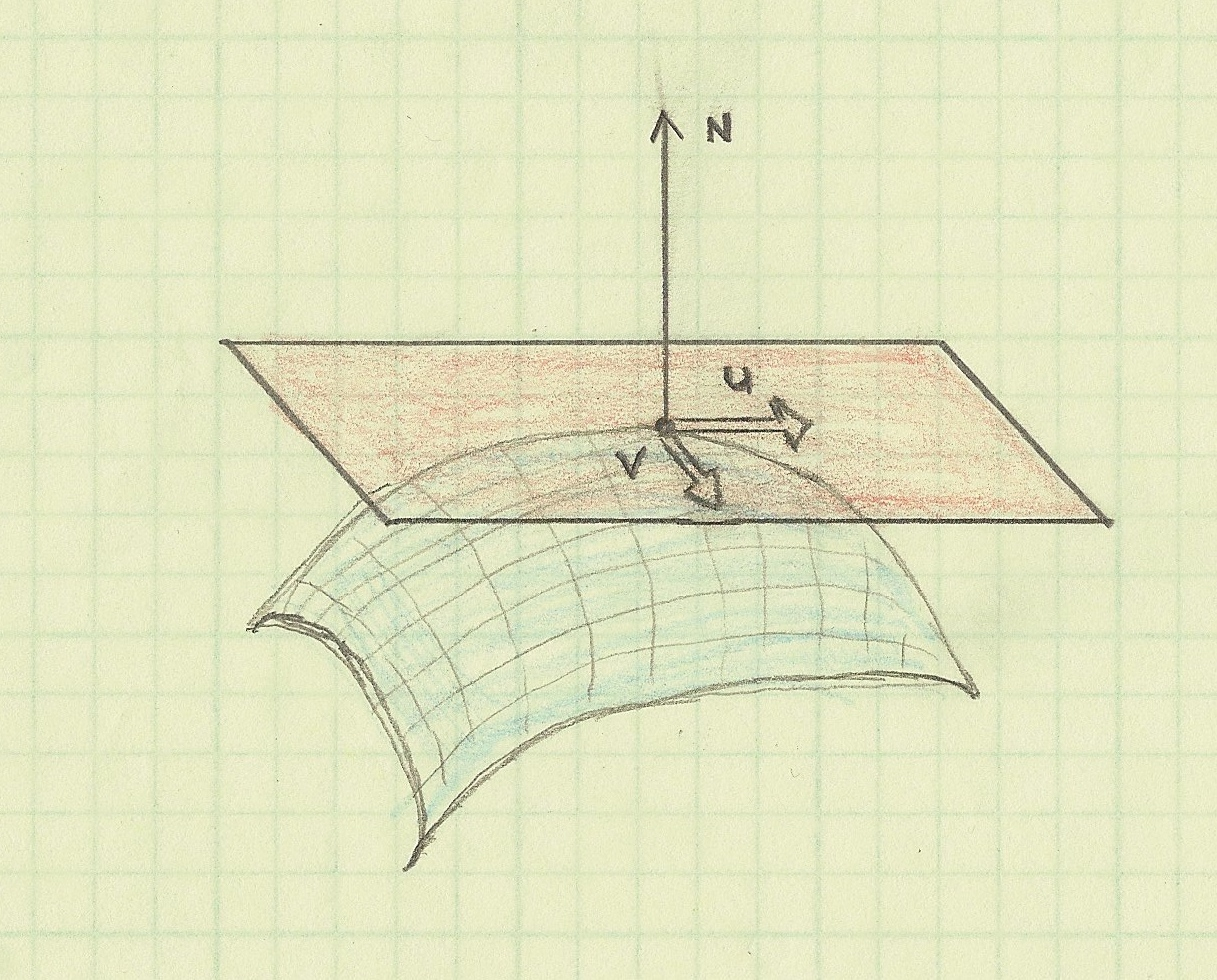
\includegraphics[scale=.11]{Pict/Tang-vect2.jpg}
    \end{center}
    It \alert{is} a 2-dimensional manifold.
    \column{.5\textwidth}
    \begin{center}
      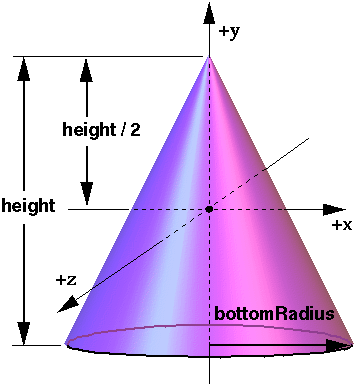
\includegraphics[scale=.3]{Pict/cone.png}
    \end{center}
    It \alert{is NOT} a 2-dimensional manifold.
  \end{columns}
\end{frame}

\begin{frame}
  \frametitle{Differentiable Maps}
  Let $M$ and $N$ be manifolds with dimensions $m$ and $n$ respectively,  $(U,\varphi)$ be a chart on $M$ and $(V,\psi)$ be charts on $N$. The map $f:M\to N$ is said to be differentiable at $p\in U$, if and only if $\psi\circ f\circ \varphi^{-1}:\R^m\to \R^n$ is differentiable at $\varphi(p)$.

  \begin{alertblock}{Diffeomorphic Manifolds}
  A couple of manifolds are said to be diffeomorphic if $\psi\circ f\circ \varphi^{-1}$ is invertible and both are $C^\infty(\R^n)$.
  \end{alertblock}
  
\end{frame}
